% !TEX root = ../Victorvan Herel2025_Thesis.tex

\chapter{Threats to Validity}\label{ch:threats}

In any empirical research, we must analysed and categorize the threats to validity of the experiments. 
The threats are classified into four categories: (1) Conclusion Validity, (2) Internal Validity, (3) Construct Validity, and (4) External Validity. 
It is important to identify and present the threat and also explain what we did to mitigate or address the threat.

Figure~\ref{fig:threats} shows a diagram of the experiment principles and where lies each threat.
Please do not use this image on the paper/thesis.
Reviewers are supposed to know where the threats lie, the figure is for students to better understand the threats.
\begin{figure}[h]
	\centering
	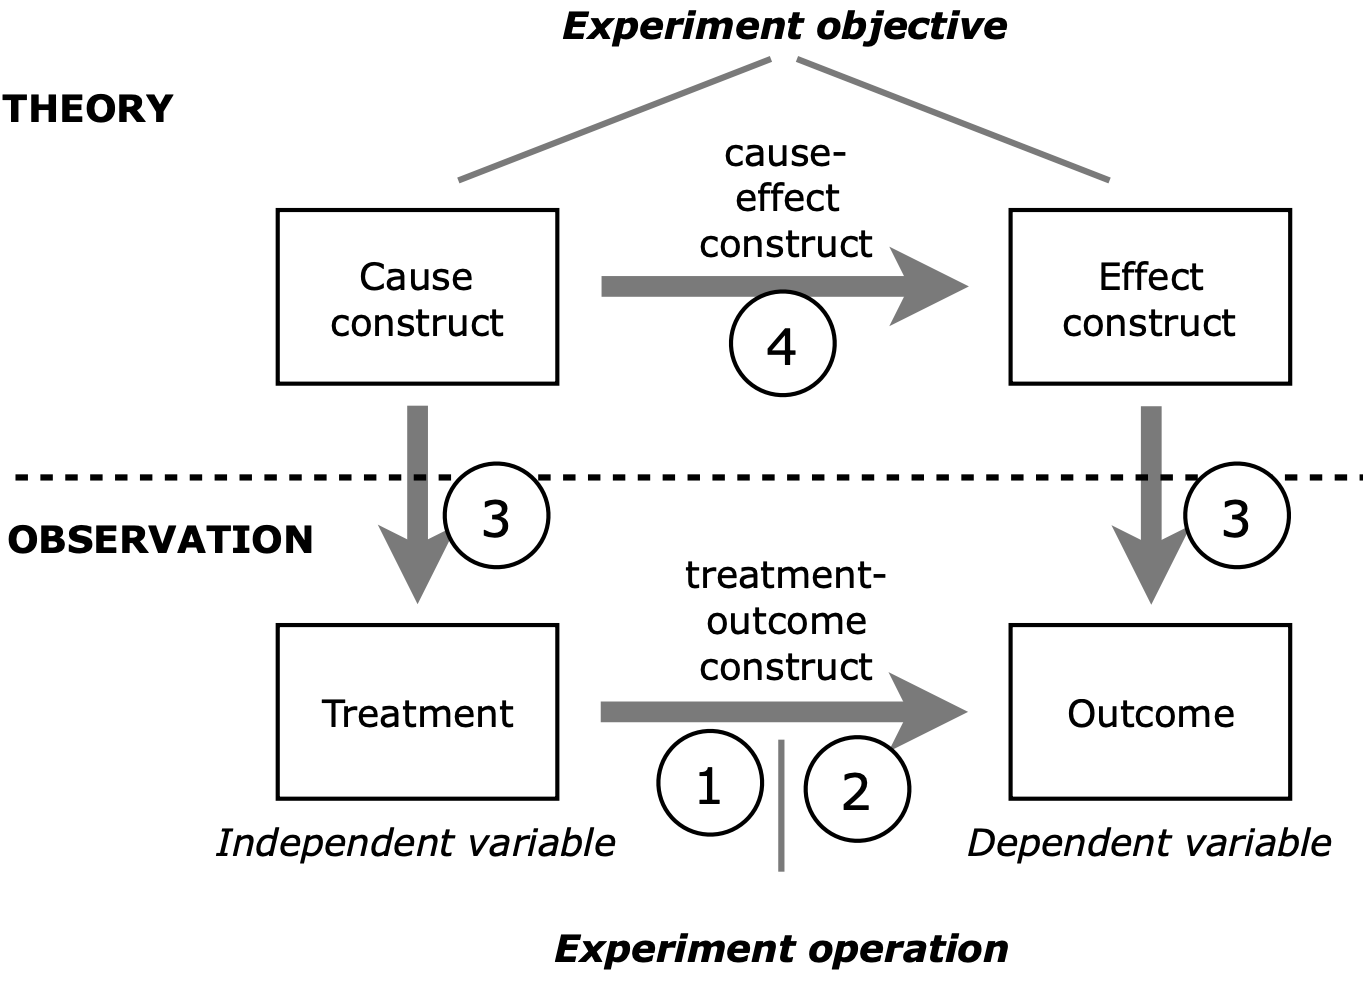
\includegraphics[width=0.75\textwidth]{images/threats-to-validity.png} 
	\caption{Experimental principles diagram showing threats. (1) Conclusion; (2) Internal; (3) Construct; and (4) External.}
	\label{fig:threats}
\end{figure}


\section{Conclusion validity}

Conclusion validity is the degree to which conclusions we reach about relationships in our data are reasonable.
\begin{itemize}
   \item  It affects the ability to draw correct conclusion about relations between treatment and outcome. \\
+ Choice of statistical tests \\
+ Choice of sample size \\
+ Measurement of the experiment
  \item Low Statistical Power \\
+ If power is low, there is a high risk that an erroneous conclusion is drawn.
\end{itemize}

\section{Internal validity}

Are there any other factors that may affect the results?
\begin{itemize}
  \item Were phenomena observed under special conditions \\
+ in the lab, close to a deadline, company risked bankruptcy, … \\
+ major turnover in team, contributors changed (open-source), …
  \item Similar observations repeated over time (learning effects)
  \item Correlation does not imply causation.
\end{itemize}

\section{Construct validity}

Do the operational measures reflect what the researcher had in mind?
\begin{itemize}
  \item Time recorded vs. time spent
  \item Execution time, memory consumption, … \\
+ noise of operating system, sampling method
  \item Human-assigned classifiers (bug severity, …) \\
+ risk for “default” values
  \item Participants in interviews have pressure to answer positively 
\end{itemize}

\section{External validity}

To what extent can the findings be generalized?
\begin{itemize}
  \item Does it apply to other languages? Other sizes? Other domains? Other systems?
  \item Background \& education of participants
  \item Simplicity \& scale of the team \\
+ small teams \& flexible roles vs. large organizations \& fixed roles
\end{itemize}